\documentclass[a4paper,11pt,fleqn,twoside,openright]{memoir} 	% Openright aabner kapitler paa hoejresider (openany begge)

%%%% PACKAGES %%%%

% ¤¤ Oversaettelse og tegnsaetning ¤¤ %
%tilføjet af AT
\usepackage{url}
\usepackage{rotating}
\usepackage{pdflscape}

\usepackage[utf8]{inputenc}					% Input-indkodning af tegnsaet (UTF8)
\usepackage[danish]{babel}					% Dokumentets sprog
\usepackage[T1]{fontenc}					% Output-indkodning af tegnsaet (T1)
\usepackage{ragged2e,anyfontsize}			% Justering af elementer
\usepackage{fixltx2e}						% Retter forskellige fejl i LaTeX-kernen	
								\usepackage{blindtext}	
								
% ¤¤ Figurer og tabeller (floats) ¤¤ %
\usepackage{graphicx} 						% Haandtering af eksterne billeder (JPG, PNG, PDF)
\usepackage{multirow}                		% Fletning af raekker og kolonner (\multicolumn og \multirow)
\usepackage{colortbl} 						% Farver i tabeller (fx \columncolor, \rowcolor og \cellcolor)
\usepackage[dvipsnames]{xcolor}				% Definer farver med \definecolor. Se mere: http://en.wikibooks.org/wiki/LaTeX/Colors
\usepackage{flafter}						% Soerger for at floats ikke optraeder i teksten foer deres reference
\let\newfloat\relax 						% Justering mellem float-pakken og memoir
\usepackage{float}							% Muliggoer eksakt placering af floats, f.eks. \begin{figure}[H]
%\usepackage{eso-pic}						% Tilfoej billedekommandoer paa hver side
%\usepackage{wrapfig}						% Indsaettelse af figurer omsvoebt af tekst. \begin{wrapfigure}{Placering}{Stoerrelse}
%\usepackage{multicol}         	        	% Muliggoer tekst i spalter
%\usepackage{rotating}						% Rotation af tekst med \begin{sideways}...\end{sideways}
\usepackage{longtable}

% ¤¤ Matematik mm. ¤¤
\usepackage{amsmath,amssymb,stmaryrd} 		% Avancerede matematik-udvidelser
\usepackage{mathtools}						% Andre matematik- og tegnudvidelser
\usepackage{textcomp}                 		% Symbol-udvidelser (f.eks. promille-tegn med \textperthousand )
\usepackage{siunitx}						% Flot og konsistent praesentation af tal og enheder med \si{enhed} og \SI{tal}{enhed}
\sisetup{output-decimal-marker = {,}}		% Opsaetning af \SI (DE for komma som decimalseparator) 
\usepackage[version=3]{mhchem} 				% Kemi-pakke til flot og let notation af formler, f.eks. \ce{Fe2O3}
%\usepackage{rsphrase}						% Kemi-pakke til RS-saetninger, f.eks. \rsphrase{R1}

% ¤¤ Referencer og kilder ¤¤ %
\usepackage[danish]{varioref}				% Muliggoer bl.a. krydshenvisninger med sidetal (\vref)
\usepackage{natbib}							% Udvidelse med naturvidenskabelige citationsmodeller
%\usepackage{xr}							% Referencer til eksternt dokument med \externaldocument{<NAVN>}
%\usepackage{glossaries}					% Terminologi- eller symbolliste (se mere i Daleifs Latex-bog)

% ¤¤ Misc. ¤¤ %
\usepackage{listings}						% Placer kildekode i dokumentet med \begin{lstlisting}...\end{lstlisting}
\usepackage{lipsum}							% Dummy text \lipsum[..]
\usepackage[shortlabels]{enumitem}			% Muliggoer enkelt konfiguration af lister
\usepackage{pdfpages}						% Goer det muligt at inkludere pdf-dokumenter med kommandoen \includepdf[pages={x-y}]{fil.pdf}	
\pdfoptionpdfminorversion=6					% Muliggoer inkludering af pdf dokumenter, af version 1.6 og hoejere
\pretolerance=2500 							% Justering af afstand mellem ord (hoejt tal, mindre orddeling og mere luft mellem ord)

% Kommentarer og rettelser med \fxnote. Med 'final' i stedet for 'draft' udloeser hver note en error i den faerdige rapport.
\usepackage[footnote,draft,danish,silent,nomargin]{fixme}		


%%%% CUSTOM SETTINGS %%%%

% ¤¤ Marginer ¤¤ %
\setlrmarginsandblock{3.5cm}{2.5cm}{*}		% \setlrmarginsandblock{Indbinding}{Kant}{Ratio}
\setulmarginsandblock{2.5cm}{3.0cm}{*}		% \setulmarginsandblock{Top}{Bund}{Ratio}
\checkandfixthelayout 						% Oversaetter vaerdier til brug for andre pakker

%	¤¤ Afsnitsformatering ¤¤ %
\setlength{\parindent}{0mm}           		% Stoerrelse af indryk
\setlength{\parskip}{3mm}          			% Afstand mellem afsnit ved brug af double Enter
\linespread{1,1}							% Linie afstand

% ¤¤ Litteraturlisten ¤¤ %
\bibpunct[,]{[}{]}{;}{a}{,}{,} 				% Definerer de 6 parametre ved Harvard henvisning (bl.a. parantestype og seperatortegn)
\bibliographystyle{bibtex/harvard}			% Udseende af litteraturlisten.

% ¤¤ Indholdsfortegnelse ¤¤ %
\setcounter{secnumdepth}{4}		 			% Dybden af nummerede overkrifter (part/chapter/section/subsection)
\setcounter{maxsecnumdepth}{4}					% Dokumentklassens graense for nummereringsdybde
\setcounter{tocdepth}{4} 					% Dybden af indholdsfortegnelsen

% ¤¤ Lister ¤¤ %
\setlist{
  topsep=0pt,								% Vertikal afstand mellem tekst og listen
  itemsep=-1ex,								% Vertikal afstand mellem items
} 

% ¤¤ Visuelle referencer ¤¤ %
\usepackage[colorlinks]{hyperref}			% Danner klikbare referencer (hyperlinks) i dokumentet.
\hypersetup{colorlinks = true,				% Opsaetning af farvede hyperlinks (interne links, citeringer og URL)
    linkcolor = black,
    citecolor = black,
    urlcolor = black
}

% ¤¤ Opsaetning af figur- og tabeltekst ¤¤ %
\captionnamefont{\small\bfseries\itshape}	% Opsaetning af tekstdelen ('Figur' eller 'Tabel')
\captiontitlefont{\small}					% Opsaetning af nummerering
\captiondelim{. }							% Seperator mellem nummerering og figurtekst
\hangcaption								% Venstrejusterer flere-liniers figurtekst under hinanden
\captionwidth{\linewidth}					% Bredden af figurteksten
\setlength{\belowcaptionskip}{0pt}			% Afstand under figurteksten
		
% ¤¤ Opsaetning af listings ¤¤ %
\definecolor{commentGreen}{RGB}{34,139,24}
\definecolor{stringPurple}{RGB}{208,76,239}

\lstset{language=Matlab,					% Sprog
	basicstyle=\ttfamily\scriptsize,		% Opsaetning af teksten
	keywords={for,if,while,else,elseif,		% Noegleord at fremhaeve
			  end,break,return,case,
			  switch,function},
	keywordstyle=\color{blue},				% Opsaetning af noegleord
	commentstyle=\color{commentGreen},		% Opsaetning af kommentarer
	stringstyle=\color{stringPurple},		% Opsaetning af strenge
	showstringspaces=false,					% Mellemrum i strenge enten vist eller blanke
	numbers=left, numberstyle=\tiny,		% Linjenumre
	extendedchars=true, 					% Tillader specielle karakterer
	columns=flexible,						% Kolonnejustering
	breaklines, breakatwhitespace=true,		% Bryd lange linjer
}

% ¤¤ Navngivning ¤¤ %
\addto\captionsdanish{
	\renewcommand\appendixname{Appendiks}
	\renewcommand\contentsname{Indholdsfortegnelse}	
	\renewcommand\appendixpagename{Appendiks}
	\renewcommand\appendixtocname{Appendiks}
	\renewcommand\cftchaptername{\chaptername~}				% Skriver "Kapitel" foran kapitlerne i indholdsfortegnelsen
	\renewcommand\cftappendixname{\appendixname~}			% Skriver "Appendiks" foran appendiks i indholdsfortegnelsen
}

% ¤¤ Kapiteludssende ¤¤ %
\definecolor{numbercolor}{gray}{0.7}		% Definerer en farve til brug til kapiteludseende
\newif\ifchapternonum

\makechapterstyle{jenor}{					% Definerer kapiteludseende frem til ...
  \renewcommand\beforechapskip{0pt}
  \renewcommand\printchaptername{}
  \renewcommand\printchapternum{}
  \renewcommand\printchapternonum{\chapternonumtrue}
  \renewcommand\chaptitlefont{\fontfamily{pbk}\fontseries{db}\fontshape{n}\fontsize{25}{35}\selectfont\raggedleft}
  \renewcommand\chapnumfont{\fontfamily{pbk}\fontseries{m}\fontshape{n}\fontsize{1in}{0in}\selectfont\color{numbercolor}}
  \renewcommand\printchaptertitle[1]{%
    \noindent
    \ifchapternonum
    \begin{tabularx}{\textwidth}{X}
    {\let\\\newline\chaptitlefont ##1\par} 
    \end{tabularx}
    \par\vskip-2.5mm\hrule
    \else
    \begin{tabularx}{\textwidth}{Xl}
    {\parbox[b]{\linewidth}{\chaptitlefont ##1}} & \raisebox{-15pt}{\chapnumfont \thechapter}
    \end{tabularx}
    \par\vskip2mm\hrule
    \fi
  }
}											% ... her

\chapterstyle{jenor}						% Valg af kapiteludseende - Google 'memoir chapter styles' for alternativer

% ¤¤ Sidehoved ¤¤ %

\makepagestyle{Uni}							% Definerer sidehoved og sidefod udseende frem til ...
\makepsmarks{Uni}{%
	\createmark{chapter}{left}{shownumber}{}{. \ }
	\createmark{section}{right}{shownumber}{}{. \ }
	\createplainmark{toc}{both}{\contentsname}
	\createplainmark{lof}{both}{\listfigurename}
	\createplainmark{lot}{both}{\listtablename}
	\createplainmark{bib}{both}{\bibname}
	\createplainmark{index}{both}{\indexname}
	\createplainmark{glossary}{both}{\glossaryname}
}
\nouppercaseheads											% Ingen Caps oenskes

\makeevenhead{Uni}{Langerhanske Øer}{}{\leftmark}				% Definerer lige siders sidehoved (\makeevenhead{Navn}{Venstre}{Center}{Hoejre})
\makeoddhead{Uni}{\rightmark}{}{Ingeniørhøjskolen Aarhus}			% Definerer ulige siders sidehoved (\makeoddhead{Navn}{Venstre}{Center}{Hoejre})
\makeevenfoot{Uni}{\thepage}{}{}							% Definerer lige siders sidefod (\makeevenfoot{Navn}{Venstre}{Center}{Hoejre})
\makeoddfoot{Uni}{}{}{\thepage}								% Definerer ulige siders sidefod (\makeoddfoot{Navn}{Venstre}{Center}{Hoejre})
\makeheadrule{Uni}{\textwidth}{0.5pt}						% Tilfoejer en streg under sidehovedets indhold
\makefootrule{Uni}{\textwidth}{0.5pt}{1mm}					% Tilfoejer en streg under sidefodens indhold

\copypagestyle{Unichap}{Uni}								% Sidehoved for kapitelsider defineres som standardsider, men med blank sidehoved
\makeoddhead{Unichap}{}{}{}
\makeevenhead{Unichap}{}{}{}
\makeheadrule{Unichap}{\textwidth}{0pt}
\aliaspagestyle{chapter}{Unichap}							% Den ny style vaelges til at gaelde for chapters
															% ... her
															
\pagestyle{Uni}												% Valg af sidehoved og sidefod (benyt "plain" for ingen sidehoved/fod)


%%%% CUSTOM COMMANDS %%%%

% ¤¤ Billede hack ¤¤ %										% Indsaet figurer nemt med \figur{Stoerrelse}{Fil}{Figurtekst}{Label}
\newcommand{\figur}[4]{
		\begin{figure}[H] \centering
			\includegraphics[width=#1\textwidth]{billeder/#2}
			\caption{#3}\label{#4}
		\end{figure} 
}

% ¤¤ Specielle tegn ¤¤ %
\newcommand{\decC}{^{\circ}\text{C}}
\newcommand{\dec}{^{\circ}}
\newcommand{\m}{\cdot}


%%%% ORDDELING %%%%

\hyphenation{}											% Preamble indlaeses
\raggedbottom													% Soerger for at LaTeX ikke "straekker" teksten

%\includeonly{file1,file2}										% Inkluder kun specifikke filer (kommasepareret liste)

\begin{document}												% Starter dokumentet - obligatorisk


\frontmatter													% Forindhold - nummereres med romertal

\thispagestyle{empty}
\begin{center}
\vspace{3cm}

\phantom{hul}

\phantom{hul}

\phantom{hul}

\textsl{\LARGE Cell sorter for isolation of insulin producing cells} \\ \vspace{0.25cm}
\textsl{\Large Projektdokumentation} \\ %\vspace{1cm}

\rule{13cm}{3mm} \\ \vspace{1cm}


\includegraphics[width=0.9\textwidth]{billeder/forside.jpg}

\textsc{\center Bachelorprojekt \\
Projektnr: 15137 \\
Ingeniørhøjskolen, Aarhus Universitet \\
Den 16. december 2015 \\ \vspace{1cm}
11242	Anders Toft Andersen \\
201270874	Anders Esager \\
Projektvejleder: Samuel Alberg Thrysøe \\}
\end{center}

\cleardoublepage												% Indsaetter tom side, saa naeste kapitel starter paa hoejre side (hvis noedvendigt)
% Dette er et titelblad designet til videregående uddannelser på et universitet
% Filen kræver:
% Universitetets logo:  AU-logo-DK eller AU-logo-DK
% Synopsis: En fil ved navn synopsis.tex

% Udarbejdet af: Jesper Nørgaard (jesper@noergaard.eu) 10. april 2012

\phantomsection
\pdfbookmark[0]{Titelblad}{titelblad}
\thispagestyle{empty}

\begin{minipage}[t]{0.48\textwidth}
\vspace*{-8pt}			

\includegraphics[height=2.5cm]{billeder/AU-logo-DK}
\end{minipage}
\hfill
\begin{minipage}[t]{0.48\textwidth}
{\small 
\textbf{Studienævn for Aarhus School of Science}\\
Nordre Ringgade 1 \\
8000 Aarhus C \\
Tlf: 8715 0000 \\
http://www.au.dk}
\end{minipage}

\vspace*{1cm}

\begin{minipage}[t]{0.48\textwidth}
\textbf{Titel:} \\[5pt]\bigskip\hspace{2ex}
Energirenovering

\textbf{Projekt:} \\[5pt]\bigskip\hspace{2ex}
P1-projekt

\textbf{Projektperiode:} \\[5pt]\bigskip\hspace{2ex}
September 2014 - December 2014

\textbf{Projektgruppe:} \\[5pt]\bigskip\hspace{2ex}
B131	

\textbf{Deltagere:} \\[5pt]\hspace*{2ex}
Adam  G. Hansen \\\hspace*{2ex}
Berit Jørgensen \\\hspace*{2ex}
Christoffer Haning \\\hspace*{2ex}
Dorthe Møller \\\hspace*{2ex}
Ejnar V. Jensen \\\hspace*{2ex}
Freja Poulsen \\\bigskip\hspace{2ex}
Gerhard Pedersen

\textbf{Vejledere:} \\[5pt]\hspace*{2ex}
Carsten Henningsen \\\bigskip\hspace{2ex}
Lotte Dalgaard

\vspace*{1cm}

\textbf{Oplagstal: 10} \\
\textbf{Sidetal: 80} \\
\textbf{Appendiks: 3} \\ 
\textbf{Afsluttet 18-12-2014}

\end{minipage}
\hfill
\begin{minipage}[t]{0.483\textwidth}
Synopsis: \\[5pt]
\fbox{\parbox{7cm}{\bigskipSynopsis

\bigskip}}
\end{minipage}

\vfill

{\footnotesize\itshape Rapportens indhold er frit tilgængeligt, men offentliggørelse (med kildeangivelse) må kun ske efter aftale med forfatterne.}

% Rapportens indhold er frit tilgængeligt, men offentliggørelse (med kildeangivelse) må kun ske efter aftale med forfatterne.
% The content of the report is freely available, but publication (with source reference) may only take place in agreement with the authors.

\cleardoublepage
\chapter*{Forord}

Denne rapport er udarbejdet som en del af syvende semesters bachelorprojekt på Ingeniørhøjskolen, Aarhus Universitet. Rapporten er udarbejdet af en projektgruppe bestående af 2 sundhedsteknologistuderende. Projektet er udarbejdet i samarbejde med Søren Gregersen, overlæge på Medicinsk Endokrinologisk Afdeling på Aarhus Universitetshospital med hjælp fra Per. B. Jeppesen, Lektor ved Institut for Klinisk Medicin, Aarhus Universitet. Bachelorprojektet er udført i perioden 28. august 2015 til 16. december 2015, hvor forprojektet er udført i perioden 26. april 2015 til 15. juni 2015.  

Projektgruppen retter en stor tak til Søren Gregersen for samarbejdet, ligeledes skal der gives en tak til Per B. Jeppesen. Ydermere skal der lyde en varm tak til gruppens vejleder Samuel Thrysøe, der har hjulpet og støttet gruppen igennem hele processen. Endelig skal der gives en tak til reviewgruppen bestående af Simon Vammen Grønbæk og Karl-John Schmidt, som har bestået med konstruktiv kritik og rettelser. 


%Dette dokument indeholder projektdokumentationen for projektet \textit{Cell sorter for isolation of insulin producing cells}. Dokumentet indeholder kravspecifikation og accepttest for systemet, samt beskrivelse af projektets design og implementeringsfase. 

%Kravspecifikationen er udarbejdet i samarbejde med Søren Gregersen, overlæge på Medicinsk Endokrinologisk Afdeling, Aarhus Universitetshospital, der agerer som projektets kunde. 



\phantom{Luft}

\phantom{Luft}

\begin{table}[H]
	\centering
		\begin{tabular}{c c}
			\underline{\phantom{mmmmmmmmmmmmmm}} & \underline{\phantom{mmmmmmmmmmmmmm}}  \\
			Anders Toft Andersen			& Anders Esager		 			\\ 										\end{tabular}
\end{table}

\section*{Læsevejledning}
Rapporten indeholder primært metoder, resultater og diskussioner til produktet, som gruppen har udarbejdet. Der vil igennem rapporten fremtræde kildehenvisninger, og disse vil være samlet i en kildeliste bagerst i rapporten. Der er i rapporten anvendt kildehenvisning efter Harvardmetoden, i teksten refereres en kilde med [Efternavn, År]. Denne henvisning fører til kildelisten, hvor bøger er angivet med forfatter, titel, udgave og forlag, mens internetsider er angivet med forfatter, titel og dato. Til sidst i rapporten er bilagsliste, som anskueliggør filnavnene i den afleverede bilagsmappen. Diagrammerne udarbejdet i projektet er skrevet på engelsk. 

I bilagslisten forefindes alle filerne, der er afleveret ved siden af rapporten, herunder datablade, Matlab-kode, Eagle kilde-filer og Gerber-filer. Herudover er den udfyldte accepttest og fejlrapport vedlagt som bilag.

Ved siden af rapporten er vedlagt en video, som viser den udviklede prototype.

%Der vil igennem rapporten fremtræde kildehenvisninger, og disse vil være samlet i en kildeliste bagerst i rapporten. Der er i rapporten anvendt kildehenvisning efter Harvardmetoden, så i teksten refereres en kilde med [Efternavn, År]. Denne henvisning fører til kildelisten, hvor bøger er angivet med forfatter, titel, udgave og forlag, mens Internetsider er angivet med forfatter, titel og dato. Figurer og tabeller er nummereret i henhold til kapitel, dvs. den første figur i kapitel 7 har nummer 7.1, den anden, nummer 7.2 osv. Forklarende tekst til figurer og tabeller findes under de givne figurer og tabeller.

\cleardoublepage

%%%% Indholdsfortegnelse (TOC) %%%%

\phantomsection													% Kunstigt afsnit, som hyperlinks kan 'holde fast i'
\pdfbookmark[0]{Indholdsfortegnelse}{indhold}					% Tildeler en klikbar bookmark til den endelige PDF
\tableofcontents*												% Indholdsfortegnelsen (kaldet ToC) 

%\addtocontents{toc}{\protect\newpage}							% Fremtvinger sideskift i ToC hvis noedvendig (der hvor koden placeres)


\mainmatter														% Hovedindhold - nummereres fra side 1

%%%% Rapportindhold %%%% 										% Rapportindholdet boer IKKE indeholde broedtekst - KUN includede filer!

%% Indledende %%												% Opdel evt. i passende afsnit for overblikkets skyld

\section{Indledning}
Dette dokument indeholder accepttesten for the Cell Collector(omtales herefter som systemet). 

\subsection{Formål}
Formålet med dokumentet er at sikre at alle krav til produktet er opfyldt, i henhold til kravspecifikationen.

\chapter{Projektbeskrivelse}

Projektforslaget lægger op til at belyse effekterne af energirenovering samt hvordan barrierne overvindes ved brug af virkemidler. 

I det følgende reflekteres der over emnerne i problemanalysen. Problemformuleringen indrammer herefter projektet inden det konkretiseres i afgrænsningen. Endelig beskrives de metoder, som søges anvendt. 

\section{Problemanalyse}

\section{Problemformulering}

I den kontekstuelle del søges følgende spørgsmål besvaret.

I den tekniske del søges følgende energi- og konstruktionsmæssige spørgsmål besvaret.

\section{Projektafgrænsning}

\section{Metode}
\chapter{Kravspecifikation}

\section{Indledning}
Dette dokument indeholder kravspecifikationen for The Cell Collector(omtales herefter som systemet). Dokumentet er udarbejdet i samarbejde med kunden(Søren Gregersen) og specificerer kundens kvalitetskrav, samt funktionelle og ikke funktionelle krav. Der er sammen med kunden udarbejdet en accepttest, som har til formål at teste de specificerede krav i kravspecifikation.
\section{Versionshistorik}
Tabel...

\section{Systembeskrivelse}
Formålet med projektet er at udvikle et system til isolation af insulin producerende celler (Langerhanske Øer). Mange farmaceutiske virksomheder og forskningsafdelinger udfører forsøg på disse øer fra bl.a. rotter. Processen med isolering af Langerhanske øer startes ved operativt at fjerne pancreas, hvorefter vævet opløses vha. enzymet kollagenase. Når vævet er opløst fortyndes det yderligere inden det hældes i petriskåle. Øerne bliver herefter manuelt isoleret vha. mikroskop og diverse præcisions redskaber. Denne proces er både besværlig og tidskrævende. Formålet med projektet er derfor, at udvikle en ny metode til isolation af cellerne. Systemet skal indeholder en beholder til opløsningen med langerhanske øer. Denne opløsning skal føres ud gennem en tynd slange(<0,5mm)  forbi et kamera, hvor der ved hjælp af Matlab skal udføres billedprocessering. Billedebehandlingen skal genkende, hvornår der er en langerhanske ø. Derefter skal systemet frasortere denne, ved et ventil system der åbner på det rigtige tidspunkt. Til at skabe flowet i slangerne anvendes en pumpe.  Et krav til pumpen er at den skal være nænsom ved celleopløsningen, da de langerhanske øer er meget skrøbelige.
En automatiseret løsning af sorteringsprocessen kan bidrage med reducering af omkostningerne, give en mere ensartet sortering samt sikre dokumentation af de sorterede øer. Systemet kan fra et kommercielt synspunkt bidrage til basal forskning og til screening af nye medicinske præparater.

Indsæt figur!!
\section{Funktionelle krav}
\subsection{Aktør beskrivelse}
Systemets primære aktør er operatøren, som står for påfyldning af celler, start og stop af sorteringsprocessen. Operatøren har mulighed for at interagere med systemet via en grafisk brugergrænseflade. Systemets sekundære aktør er PC’ens filsystem, hvor der løbende gemmes en log over sorteringsprocessen.
\subsection{Use Case Diagram}
Indsæt figur!!
%\subsection{Use Case 1 - Start sorteringscyklus}
\label{uc:1}
\begin{center}
		\begin{longtable}{ | m{4cm} | m{8cm}| } 
			\hline
			Mål & Start sorteringscyklus \\ 
			\hline
			Initiering &  Use casen initieres af operatøren\\
			\hline
			Aktør & 
			Primær: Operatør
			
			 Sekundær: Kamera			  \\ 
			\hline
			Startbetingelser & The Cell Collector programmet er startet på computeren \\ 
			\hline	
			Slutbetingelser ved succes & Systemet starter med sorteringen af Langerhanske øer \\
			\hline
			Slutbetingelser ved undtagelse & N/A \\
			\hline
			Normalforløb & \begin{enumerate}
				%\setlength\itemsep{0cm} % Decrease line distance
				\item Operatør fylder celleopløsningsbeholderen
				\item Celleopløsningsbeholderen er fyldt
				\item Operatør starter sorteringscyklus ved at klikke på [Start]
				\subitem [Undtagelse 1: Wastebeholder er fyldt] 
				\item Systemet initialiserer Arduinoen
				\subitem [Undtagelse 2: Ingen forbindelse til Arduino]
				\item Systemet kontrollerer celleopløsningsbeholderen ved at konvertere spændingen (\SI{}{\volt})  til \SI{}{\milli\litre}, og vise beholderens indhold (\SI{}{\milli\litre}) på GUI
				\item Systemet initialiserer kameraet
				\subitem [Undtagelse 3: Kameraet initialiserer ikke]
				\item Systemet tænder for kamera lyset
				\item Systemet tænder for pumpen
				
			\end{enumerate} \\ 
			\hline
			Undtagelser & [Undtagelse 1: Wastebeholder er fyldt] 
			
			\begin{enumerate}
			\item Systembesked: Tøm venligst Wastebeholder før start
			\item Operatøren trykker “OK”
			\item Systemet fortsætter opstartprocessen
			\end{enumerate} 
			
			[Undtagelse 2: Ingen forbindelse til Arduino]
			
			\begin{enumerate}
			\item 1.	Systembesked: Ingen forbindelse til Arduino, kontrollér forbindelser.
			\end{enumerate} 
	
			[Undtagelse 3: Kameraet initialiseres ikke]
			
			\begin{enumerate}
			\item System fejlmeddelse: Kameraet er ikke initialiseret:
			\item Genstart initialisering af Kameraet
			\end{enumerate} \\
			\hline
		\end{longtable}
		
	\end{center}
	\pagebreak
\subsection{Use case 2 - Sortering af Langerhanske Øer}
\label{uc:2}
\begin{center}
		\begin{longtable}{ | m{4cm} | m{8cm}| } 
			\hline
			Mål & Sortere Langerhanske Øer \\ 
			\hline
			Initiering &  Use casen initieres af [UC 1: Startsorteringscyklus]\\
			\hline
			Aktør & Kamera \\ 
			\hline
			Startbetingelser & Systemet er startet og sorteringscyklussen er i gang\\ 
			\hline	
			Slutbetingelser ved succes & Systemet har isoleret en Langerhansk ø og ventilen er lukket \\
			\hline
			Slutbetingelser ved undtagelse & \\
			\hline
			Normalforløb & \begin{enumerate}
				%\setlength\itemsep{0cm} % Decrease line distance
				\item Systemet detekterer en Langerhansk ø
				\item Arduino sender signal til ventilen om åbning
				\item Ventilen åbner
				\item Arduino sender signal til ventilen om lukning
				\item Ventilen lukker
			\end{enumerate} \\ 
			\hline
			Undtagelser & \\
			\hline
		\end{longtable}
		
	\end{center}
	\pagebreak
\subsection{Use Case 3 - Stop sorteringscyklus}
\begin{center}
		\begin{longtable}{ | m{4cm} | m{8cm}| } 
			\hline
			Mål & Stop sorteringscyklus \\ 
			\hline
			Initiering &  Use casen initieres af operatøren\\
			\hline
			Aktør & Operatør \\ 
			\hline
			Startbetingelser & [UC 2: Sortering af Langerhanske Øer] er startet\\ 
			\hline	
			Slutbetingelser ved succes & [UC 2: Sortering af Langerhanske Øer] er stoppet \\
			\hline
			Slutbetingelser ved undtagelse & N/A \\
			\hline
			Normalforløb & \begin{enumerate}
				\setlength\itemsep{0cm} % Decrease line distance
				\item Operatør stopper sorteringscyklussen ved at trykke på [Stop]
				\subitem [Undtagelse 1: Tom celleopløsningsbeholder]
				\item Systemet slukker for pumpen
				\item Systemet slukker for kameraet
				\item Systemet slukker for kamera lyset
				\item Systemet slukker for Arduino
			\end{enumerate} \\ 
			\hline
			Undtagelser & TODO!!\\
			\hline
		\end{longtable}
		
	\end{center}
	\pagebreak
\subsection{Use case 4 - Indstillinger}
\begin{center}
		\begin{longtable}{ | m{4cm} | m{8cm}| } 
			\hline
			Mål & Ændre systemets indstillinger \\ 
			\hline
			Initiering &  Use casen initieres af operatør\\
			\hline
			Aktør & Operatør \\ 
			\hline
			Startbetingelser & [UC 2: Sortering af Langerhanske Øer] er endnu ikke startet\\ 
			\hline	
			Slutbetingelser ved succes & Systemets indstillinger er ændret \\
			\hline
			Slutbetingelser ved undtagelse & Systemets indstillinger er uændret \\
			\hline
			Normalforløb & \begin{enumerate}
				%\setlength\itemsep{0cm} % Decrease line distance
				\item Operatøren klikker på [Indstillinger]
				\item Et nyt vindue åbner med systemets indstillinger.
				\item Operatøren vælger de ønskede indstillinger, og trykker [Gem indstillinger]
				\subitem [Undtagelse 1: Operatøren klikker [Annuller]]
				\item Systemets indstillinger gemmes.
			\end{enumerate} \\ 
			\hline
			Undtagelser & [Undtagelse 1: Operatøren klikker “Annuller”]
			
			\begin{enumerate}
			\item Systemet lukker Indstillingsvinduet og indstillingerne er uændret.
			\end{enumerate} \\
			\hline
		\end{longtable}
		
	\end{center}
	\pagebreak


\section{Ikke funktionelle krav}
Todo: kvalitetskrav fra kunde
\subsection{Hardware}

\subsubsection{Microcontroller} \label{subsub:mcu}
\begin{enumerate}
\item Atmega328p (Arduino)
\end{enumerate}

\subsubsection{Pumpe} \label{subsub:pump}
\begin{enumerate}
\item Pumpe flow: <50ml / min 
\item Størrelse på studserne skal kunne tilpasses slangerne 
\end{enumerate}

\subsubsection{Slanger} \label{subsub:tubes}
\begin{enumerate}
\item Slangerne skal have en indre diameter > 300µm
\item Kameraet skal kunne detektere langerhanske øer igennem slangen, evt. vha. glasrør
\end{enumerate}

\subsubsection{Beholdere} \label{subsub:container}
\begin{enumerate}
\item Celleopløsningsbeholder skal have størrelse  > 250 mL
\item Wastebeholder skal have en størrelse dobbelt så stor som celleopløsningsbeholderen: > 500 mL
\end{enumerate}

\subsubsection{Ventil} \label{subsub:valve}
\begin{enumerate}
\item 3-vejs, dvs. 1 tilgang og kobling mellem 2 udgange
\item Studserne skal kunne tilpasses slangerne
\item Skal være til væske
\item Lukke og åbne tid skal være >50ms
\end{enumerate}

\subsubsection{Kamera} \label{subsub:camera}
\begin{enumerate}
\item Kameraet til kunne detektere langerhandske øer mellem 100 og 300um
\item Kameraet skal have en zoom funktion, som et mikroskop
\item Kameraet skal have et USB interface
\end{enumerate}


\subsection{Software} 

\subsubsection{Dataformat og struktur} \label{subsub:software}
\begin{enumerate}
\item CSV format med kommasepareret delimiter. 
\item Filnavn: Dato og starttidspunkt for sorteringscyklus.
\item Header indeholdende opsætningsindstillinger.
\item Filen er opbygget med følgende kolonner: 
\begin{enumerate}
\item Tidsstempel i formatet DD-MM-YYYY-hh:mm:ss
\item Ø størrelse
\item Radius
\item Omkreds
\item Middelintensitet
\end{enumerate}
\end{enumerate}



\section{Projektafgrænsning}
Til at afgrænse kravene i projektet er der anvendt MoSCoW metoden. Denne metode er brugt for at give en struktureret oversigt over hvilke krav der er vigtigst at få opfyldt inden for tidsrammen og hvilke der evt. kan implementeres senere hvis tiden er til det.

INDSÆT FIGUR!!
\section{Samarbejdspartner}
Gruppens kunde er Søren Gregersen, overlæge på Medicinsk Endokrinologisk Afdeling, Aarhus Universitetshospital. Det er i samarbejde med ham at projektet er blevet specificeret, samt hvilke krav der er til den endelige prototype.
Samuel Alberg Thrysøe er gruppens projektvejleder. Der afholdes ugentligt et vejledermøde, hvor gruppen giver status på projektet og hvor der diskuteres forskellige problemstillinger. 
Simon Vammen Grønbæk og Karl Johan Schmidt fungerer som projektets review gruppe. Der holdes møde hver anden uge omhandlende aftalt dagsorden. Formålet med review gruppen er at få konstruktiv feedback på evt. rettelser, opbygning af rapport og generel forståelse.

\include{accepttest/accepttest}
\chapter{Design}

%\section{Formål}

%\section{Overordnet}
%Overordnet BDD?

% Sekvensdiagrammer over UC

 \section{Hardware}
%metatekst til hardware
<<<<<<< HEAD
Dette afsnit skal være med til at dokumentere hardwaren i systemet \textit{the cell collector}, derfor indeholder afsnittet fysiske dele og deres funktionalitet. De fysiske deles specifikationer er udybes og beskrevet i dette dokument. Der er begrundelser og argumenter for hvorfor de brugte komponenter er valgt.

\subsection{Læsevejledning til hardware}
%læsevejledning
Da dette afsnit er en udspecificering af hvilke specifikationer hardware komponenterne består af, ligger det sig tæt op af kravspecifikationen. Da det er kravene i kravspecfikationen, der ligger til grunde for de valgte hardware dele. I afsnittet findes der forskellige diagrammer der er med til at beskrive opbygningen, og kommunikationen af delene. Til hvert diagram vil der være en kort beskrivelse af hvad det beskriver. Hvert afsnit indeholder funktionalitet, specifikationer omkring det enkle komponent og begrundelser og argumentationer hvorfor det er valgt i den skrevne rækkefølge. AFsnitter kan godt læses i dele, men for den komplette forståelse bør afsnittet læses i rækkefølge. 

%Det gamle afsnit, måske skal det være i et leverandør afsnit 
% Dette afsnit indeholder den nødvendige viden hardware delene i systemet Denne blok beskriver forbindelserne mellem diverse hardware med et internal block definition diagram. Dette diagram er med til at sikre at delene kan kommunikere sammen, uden unødvendige adaptere og omformere. Yderligere er der beskrevet hvordan information søgning, og viden er fundet omkring komponenterne. Primær kan det siges at hardware delene er fundet på Ebay.com(kilder til de konkrete sider?(måske under hvert produkt?)), for at hold budgettet i bund. Den manglende datablade og lidt tvivlsomme kvalitet er accepteret, da dette projekt først og fremmest er  ”\textit{proof of concept}” projekt.
 
 
 
=======
 Dette afsnit indeholder alt omkring hardware delene, fra hvilke krav der er gået ud fra til hvad der er fundet frem til.  Afsnittet beskriver hvordan information søgning, og viden er fundet omkring komponenterne. Primært er hardware delene  fundet på Ebay.com (kilder til de konkrete sider?(måske under hvert produkt?)), for at holde budgettet nede. De manglende datablade og tvivlsomme kvalitet er accepteret, da dette projekt først og fremmest er  ”\textit{proof of concept}” projekt.

Nedenstående blokdiagrammer (figur: \ref{fig:bdd_Hardware} og figur: \ref{fig:ibd_Hardware}) beskriver hvilke hardware blokke systemet består af, samt forbindelserne mellem disse. Diagrammerne er med til at sikre at delene kan kommunikere sammen, uden unødvendige adaptere og omformere. 
>>>>>>> origin/master
 
 
 
 
 \newpage
\subsection{Block Definition Diagram} 
Et bdd diagram giver indblik i hardwarens overordnede struktur af systemet. Hver block er en del der indgår i systemet. Diagrammet er bygget hierarkisk system, hvor en blok kan indeholde flere blokke. blokkene består af en system blok \textit{the cell collector}, der indeholder tre elementære blokke, \textit{Arduino}, \textit{non electronic} og \textit{Camera}. Hvor \textit{Arduino} er den eneste der indeholder flere blokke, det beskriver hvilken hardware de overstående blokke kommuniker med.


\begin{figure}[H]
	\centering
	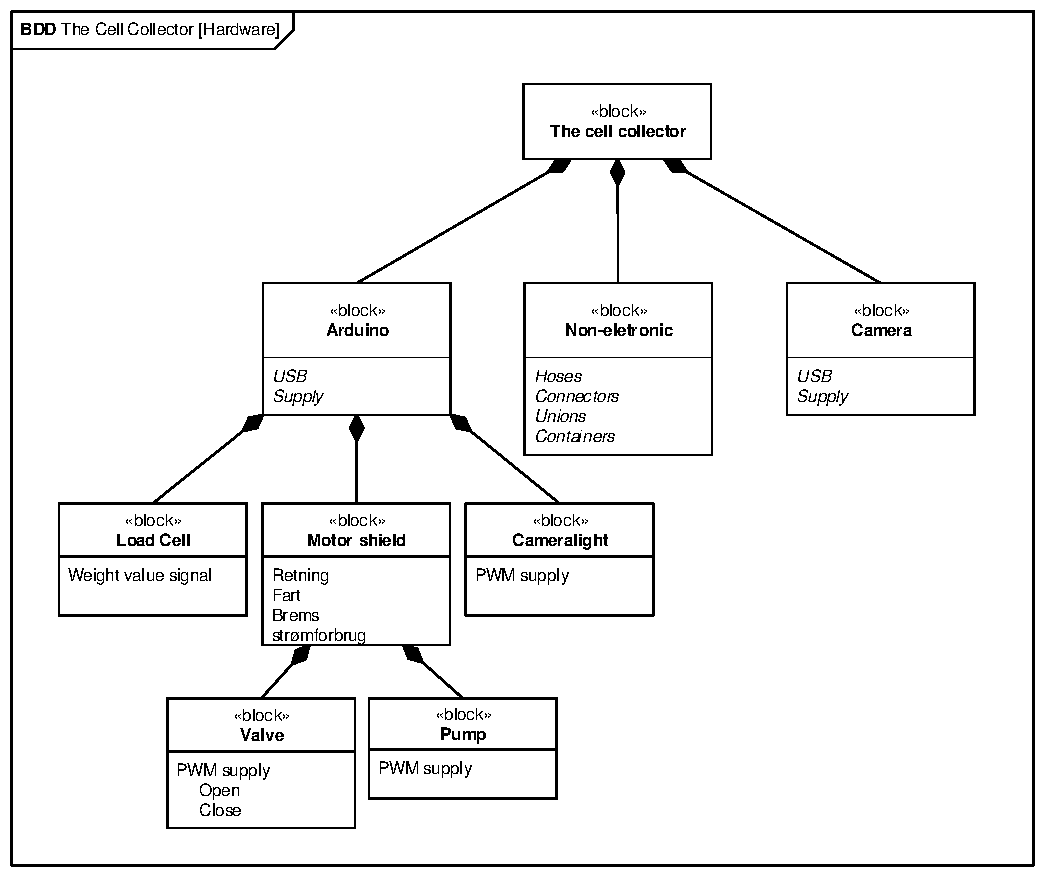
\includegraphics[width=1\textwidth]{pdf/BDD_Hardware_4315_cropped.pdf}
	\caption{BDD - Cell Collector [Hardware]}
	\label{fig:bdd_Hardware}
\end{figure}

<<<<<<< HEAD
\subsection{internal block Diagram} 
Et IBD diagram beskriver mere præcist, hvordan de forskellige komponenter med hinanden på. Det betyder at der er specialiseret indgangs- og udgangsporte, med de forskellige typer. Digrammet beskriver blandt andet, hvilken spænding delene arbejder under og hvilket signal der er brug for.
=======
\subsection{Internal block Diagram} 
>>>>>>> origin/master
\begin{figure}[H]
	\centering
	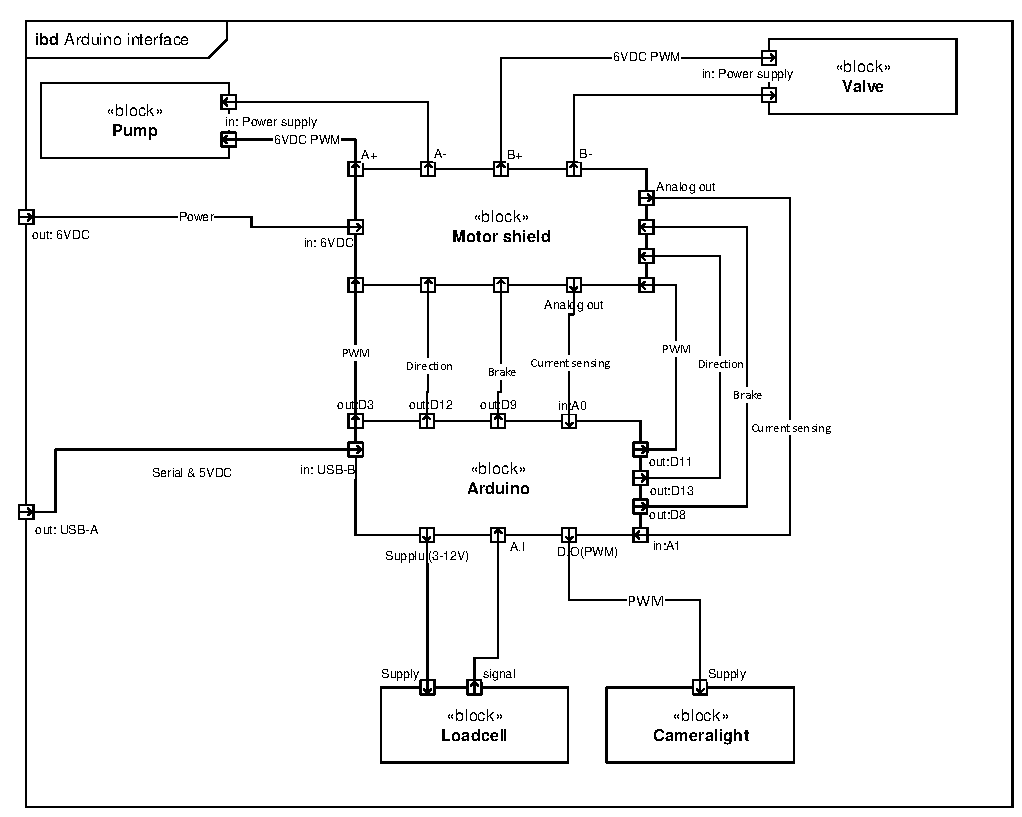
\includegraphics[width=1\textwidth]{pdf/IBD_Hardware(Arduino)_cropped.pdf}
	\caption{IBD - Cell Collector [Hardware]}
	\label{fig:ibd_Hardware}
\end{figure}



\subsection{Kamera}
Kameraet skal detektere de langerhanske øer, når de kommer forbi i slangen.  Da de langerhanske øer skiller sig ud ved at være mere lyse end resten af vævet, vil det være underordnet om kameraet er et farve kamera. Da systemet ikke skal operere under en stor hastighed er en standard frame rate valgt på 30 f/s. Kameraet opløsningen er valgt ud fra, at det skal kunne se de langerhanske øer med en størrelse på 100-300um. Til bestemmelse til dette er der brugt følgende formel:
 \fixme{Mangler formel}
For at kameraet har mulighed for, at se lidt flere detaljer og forhåbning om at det kan være tættere på end 10 cm, er det besluttet er et 2 megapixels kamera burde være passende.

\url{http://www.baslerweb.com/media/documents/BAS1408_White_paper_Camera_Selection_EN.pdf}


Da kameraet er en elementær del af systemet opsætning, blev det prioriteret, at købe det ved en mere pålidelig forhandler for at sikre en relativ god kvalitet, hvor prisen stadig lå inden for budgettet.  

Farnell
\url{http://dk.farnell.com/duratool/bw788/microscope-digital-usb-25x-200x/dp/2319420}
 
\subsection{Slanger}
Slangerne anvendes til at føre opløsningen med de langerhanske øer, i gennem systemet og bl.a. forbi kameraet. Da de største langerhanske øer, som systemet skal håndtere er 300um i diameter, er det valgt at slangerne skal have en indre diameter på 500um. Yderligere har et krav været at kameraet skal kunne se igennem slangerne, derfor er der tilkøbt et glasrør som kameraet kan se i gennem. 
%Grundet besvær med at finde en forhandler til de små mængder der skal anvendes til projektet, er der skabt kontakt til Mikrolab. Som har været en stor hjælp med at finde dele til slanger mm.

\subsection{Arduino}
Arduino er en open source platform til fremstilling af prototype print, som kan bruge til at styre forskellige systemer som dette. Arduino platformen er valgt da Matlab understøtter interaktion via en Support package. Boardet er brugt i et stort omfang omkring i verden. Derfor er det en platform der er nemt tilgængelig og forholdsvis prisvenlig, samt at der findes en stor mængde dokumentation omkring emnet. Da det som sagt er en open source platform, kan der købes forskellige versioner. 
Arduinoen skal bruges til at styre pumpen ved hjælp af ”mini motor drive shield”. Shielded anvendes for at være sikker på at der leveres effekt nok til pumpen. Yderligere har det den fordel at strømmen til pumpen kan måles og at den er galvanisk adskilt fra forsyningen til arduinoen. Dette er dog ikke arduinoen eneste opgave den skal blandt andet også styre ventilen til sortering og lyset til kameraet.

%Det er valgt at bruge en arduino som controller for at spare tid, i forhold til selv at lave et print med en microcontroller.
%Microcontrolleren der sidder på denne version er et gruppen har brugt, og arbejdet med til et tidligere projekt. Hvilket også betyder at den allerede er i gruppen beholdning af produkter.

\subsection{Ventil}
Ventilens funktion er at sorterer de langerhanske øer fra resten af opløsningen. Der findes utrolig mange typer af ventiler, med ret store prisforskelle. Ventilen er en vigtig del af systemets hardware, da det er dens ansvar at sortere de detekterede øer fra resten af væsken. Det er svært at finde ventiler med 500um studser. Det kan godt lade sig gøre at få adaptere så større ventiler kan bruges, men sporbarheden omkring hvor den enkelte ø befinder sig, bliver svært hvis kammeret pludseligt bliver stort. Dette er et stykke hardware, hvor der kan bruges meget tid og mange penge.
Kravene til ventilen er, at den skal være 3 vejs 1 tilgang og 2 udgange, yderligere skal studserne kunne tilpasses slange størrelsen, være til væske og have en lukke/åbne tid under 50ms.

\subsection{Pumpe}
Pumpen skal skabe det nødvendige flow i væsken fra det ene punkt til det andet. Flowet skal være lavt nok til at kameraet kan nå at detekterer en ø. Herfor er det et krav at pumpens flow hastighed er variabel, så flowet kan justeres. Der findes mange forskellige typer pumper til formålet, herunder stempel pumper, peristaltiske pumper og vakuum pumper. Der er bestilt en peristaltisk pumpe som virker ved at klemme på slangen og derved skabe et flow, det er dog uvist hvordan de langerhanske øer vil opfører sig ved sådan en pumpe. Der er også købt en vakuum pumpe, som muligvis kan sidde efter ventilen. Der skal dog stadig skabes et flow til de sorterede øers beholder, måske en kombination vil være det optimale. En modultest af de enkelte pumper skal afgøre hvilken løsning der er den mest optimale. 

\subsubsection{Vakuumpumper}
\url{ http://www.ebay.com/itm/281571300037}

\url{http://www.ebay.com/itm/161665897119?_trksid=p2054502.m570.l4467&_trkparms=gh1g%3DI161665897119.N19.S2.M-4218.R1.TR2}

\subsubsection{Peristaltiskepumper}

\url{http://www.ebay.com/itm/6V-Peristaltic-Pump-Dosing-Water-Pump-DC-Motor-Tube-For-Aquarium-Lab-Analytical-/131367703927?hash=item1e96201577}

%Ligesom ved ventilen er det også et produkt der kan få budgettet til at skride, derfor er der igen gået på kompromis og brug ebay forhandlere som leverandører.

\subsection{Beholdere}
Systemet består af tre beholdere der hver i især har sin egen funktion. Den første kaldes celleopløsningbeholderen, som skal indeholde den usorteret opløsning med de langerhanske øer. Beholder nummer to kaldes isolerede langerhanske øer beholderen, som er den beholder hvor de isolerede øer samles i. Den tredje beholder er waste beholderen, den skal have resten af opløsningen som ikke består af langerhanske øer. Størrelses kravene til beholderne er at opløsningsbeholderen skal mindst være 250ml, da det er den største mængde opløsning der vil blive brugt. Wastebeholderen skal således være dobbelt så stor, så der kan køres to sorterings cyklusser uden at skulle tømme beholderen i mellem. Den isolerede beholder, skal blot kunne rumme mængden af de isolerede øer. Da projektet som tidligere nævnt er et ”proof of concept” er den eneste beholder der er hentet informationer om opløsningsbeholderen. Den bør være støvtæt, uden at være lufttæt da der ellers vil dannes et vakuum i beholderen. Derudover vil det være en fordel hvis den er forholdsvis robust, så den kan køles ned osv. på et senere tidspunkt.

\subsection{Loadcell}
Loadcellen eller vægtcellen som det kan kaldes på dansk, skal bruges til at kontrollere om der er væske i celleopløsningsbeholderen. Den indkøbte vægtcellen kan veje op til 1 kg, hvilket fint dækker vægten for celleopløsningsbeholderen.

\url{http://www.ebay.com/itm/281311660424}

%Det vil sige hvs operatøren ikke har fyldt noget i beholderen, kan der gives en systembesked omkring dette. Det mest optimale er at der hele tiden er væske i slangerne i systemet, det er det vægtcellen skal hjælpe med.


\newpage
\section{Software}
Softwaren til \textit{The Cell Collector} udvikles i Matlab. Programmet udvikles af modulær kode, der afgrænser de enkelte funktionaliteter. Ved objektorienteret programmering beskrives koden typisk vha. klassediagrammer og 3-lags modellen, hvor de enkelte klassers ansvar og grænseflader tydeligt er defineret. Da Matlab kode er opdelt i funktioner fremfor for klasser er modellen ikke velegnet. I stedet beskrives softwaren vha. blokdiagrammer, hvor funktionernes opbygning og relationer med hinanden er vist. 

Blokdiagrammet (figur: \ref{fig:bdd_software}) viser hvordan programmet er opdelt i blokke, som afgrænser de enkelte funktionaliteter. Blokkene i det nederste lag skal ses som ækvivalente til funktioner i Matlab.  
De overordnede blokke i programmet er:
\begin{itemize}
\item Arduino
\item Kamera
\item User Interface
\end{itemize}

Disse blokke er nærmere beskrevet under hver deres afsnit.

\begin{figure}[H]
	\centering
	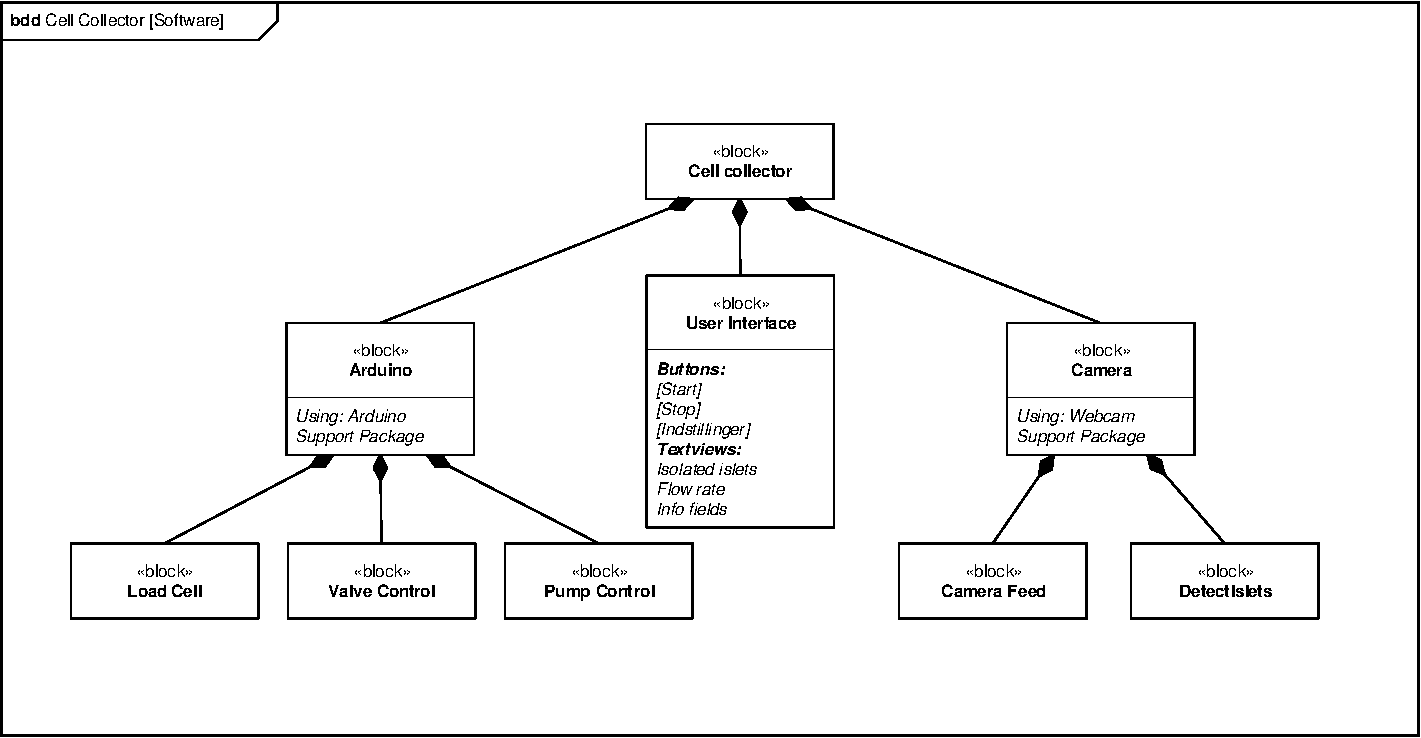
\includegraphics[width=1\textwidth]{billeder/BDD_Software-crop.pdf}
	\caption{BDD - Cell Collector [Software]}
	\label{fig:bdd_software}
\end{figure}


\subsection{Arduino}
Denne bloks formål er, at håndtere al funktionalitet til styring af Arduinoen. Til styring af Arduinoen anvendes Arduino Support Package, som frit kan hentes hos Mathworks. Den indeholder basale funktioner til bl.a. opsamling af analoge signaler, understøttelse af digitalt og PWM output og styring af DC motorer. Support biblotektet indeholder de funktioner der skal til for at styre systemets hardware.
For at initialisere Arduinoen og hardwaren implementeres en funktion, som opsætter Arduinoen med de inputs og outputs der er specificeret under hardware afsnittet (figur: \ref{ibd_Hardware}, s. \pageref{fig:ibd_Hardware}). Denne funktion er kaldt initArduino. Når brugeren klikker "Stop" skal systemet lukke ned som specificeret i Use Case 3: Stop sorteringscyklus (s. \pageref{uc:3}). Til dette implementeres en funktion kaldet stopArduino. 

\newpage

Arduino blokken er yderligere opdelt i 3 underkategorier, som vist i figur \ref{fig:bdd_software}. I det interne blok diagram (figur: \ref{fig:ibd_software_arduino}) ses underblokkenes relationer med hinanden. Disse blokke er nærmere beskrevet herunder.  
\begin{figure}[H]
	\centering
	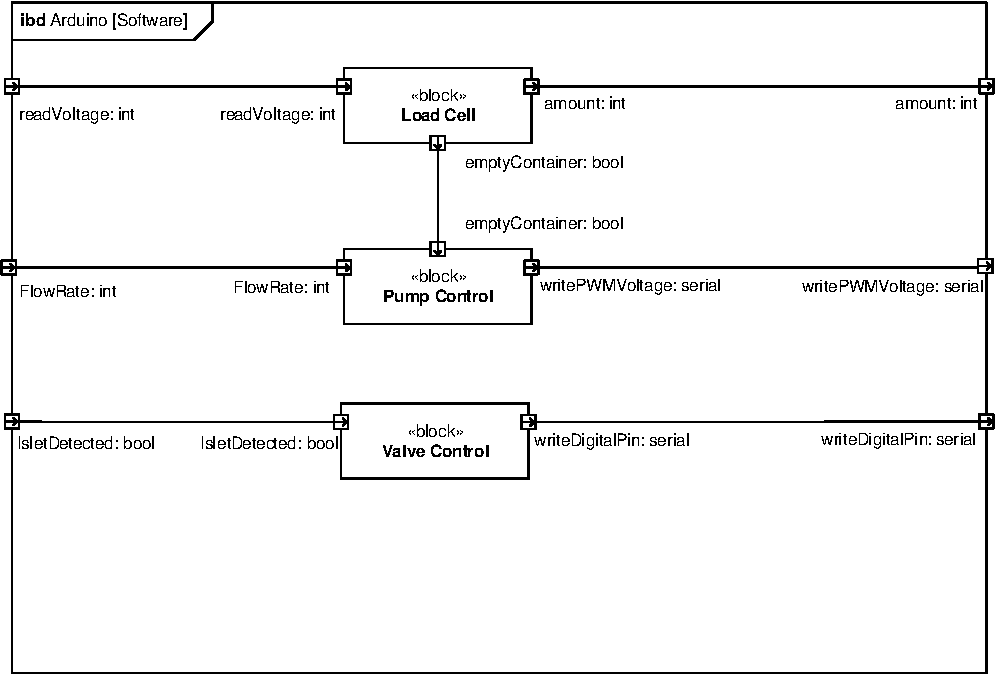
\includegraphics[width=1\textwidth]{billeder/IBD_Software_Arduino-crop.pdf}
	\caption{IBD - Arduino [Software]}
	\label{fig:ibd_software_arduino}
\end{figure}
\subsubsection{LoadCell}
Denne funktion anvendes til, at få feedback fra loadcellen. Den læser det analoge input fra Arduinoen og sammenligner den med grænseværdien for hvornår celleopløsningsbeholderen er tom. Funktionens output er en boolean, som enten er true eller false alt efter om celleopløsningsbeholderen er tom.
\subsubsection{Pump Control}
I denne funktion implementeres alt funktionalitet til styring af pumpen. Funktionen har en integer værdi som input, der specificerer flow hastigheden. Output af funktionen er et PWM moduleret signal til, at justere hastigheden på pumpen. Til dette anvendes funktionen writePWMVoltage fra Arduino Support pakken.
\subsubsection{Valve Control}
Funktionen til styring af ventilen har en boolean som input. Denne værdi indikerer om en Langerhansk Ø er detekteret af kameraet. Alt efter værdien af denne sættes forbindelsen til ventilen høj eller lav med funktionen writeDigitalPin. 

\newpage
\subsection{Kamera}
Denne bloks formål er, at modtage et feed fra kameraet samt at detektere om en Langerhansk Ø har passeret kameraet. Som det ses på det overordnede blok diagram for softwaren (figur: \ref{fig:bdd_software}) består kamera blokken af 2 underblokke. Nedenstående interne blok diagram (figur: \ref{fig:ibd_software_camera}) viser, hvordan disse blokke er forbundet internt. De enkelte blokkes funktion er yderligere beskrevet herunder.
\begin{figure}[H]
	\centering
	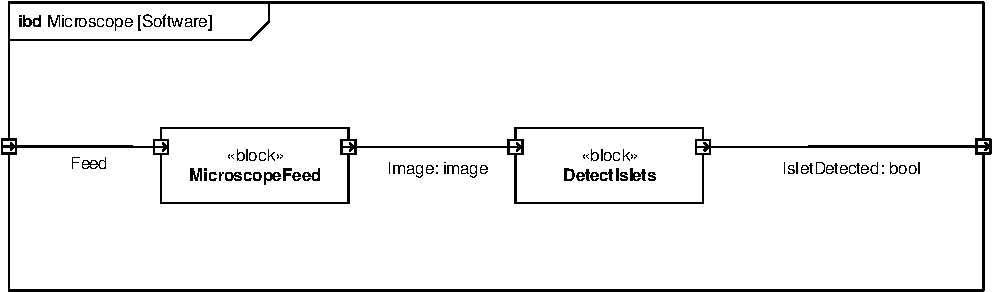
\includegraphics[width=1\textwidth]{billeder/IBD_Software_Kamera-crop.pdf}
	\caption{IBD - Camera [Software]}
	\label{fig:ibd_software_camera}
\end{figure}

\subsubsection{CameraFeed}
Denne bloks funktion er at modtage feedet fra kameraet og gemme billedet i handles. Til dette anvendes funktionen snapshot, der gemmer det nuværende billede som en variabel.  
\subsubsection{DetectIslets}
I denne funktion foregår alt billedbehandlingen på det omsamlede billede. Billedet segmenteres for at fjerne støj og andet væv. Alt efter om en Langerhansk Ø er detekteret eller ej returneres true eller false. 

\newpage
\subsection{Funktioner}
I nedenstående liste er systemets funktioner opsummeret. 
\begin{itemize}
\item initArduino
\item pumpControl 
\item valveControl 
\item loadCell 
\item cameraFeed 
\item detectIslets 
\end{itemize}
Herudover skal systemets indstillinger kunne ændres, samt data om sorteringscyklussen skal logges. Til dette implementeres funktionerne settings og exportData 
\begin{itemize}
\item settings 
\item exportData 
\end{itemize}

\newpage
\subsection{User Interface}
\subsubsection{Hovedvindue}
I figur \ref{fig:gui} er et Mockup af GUI'en vist. I venstre side er der placeret en \textit{Start knap}, som skifter stadie til en \textit{Stop knap} når den er klikket. Under denne knap er en række indikatorer placeret til, at give operatøren feedback om status omkring initialiseringen af Hardwaren. 
I højre side af GUI'en er der placeret tekstfelter til, at give brugeren feedback omkring den nuværende sorteringscyklus, samt de anvendte indstillinger. Under disse felter er en knap til \textit{Indstillinger}. Når denne klikkes åbnes et nyt vindue, hvor operatøren kan ændre i indstillingerne. 
\begin{figure}[H]
	\centering
	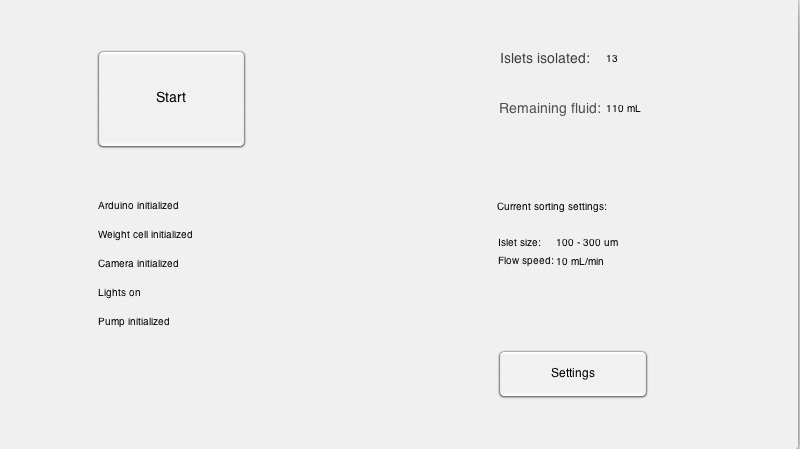
\includegraphics[width=1\textwidth]{billeder/GUI.png}
	\caption{Mockup af GUI}
	\label{fig:gui}
\end{figure}

\newpage
\subsubsection{Indstillinger}
I figur \ref{fig:gui_settings} er et Mockup af \textit{Indstillingsvinduet} vist. Via 2 tekstfelter har operatøren mulighed for, at ændre størrelsen for de celler som systemet skal sorterer. Herudover har operatøren via en dropdown menu mulighed for at ændre flowhastigheden for pumpen. I Indstillingsvinduet er der yderligere placeret en "Annuller" knap og en "Gem Indstillinger" knap.
\begin{figure}[H]
	\centering
	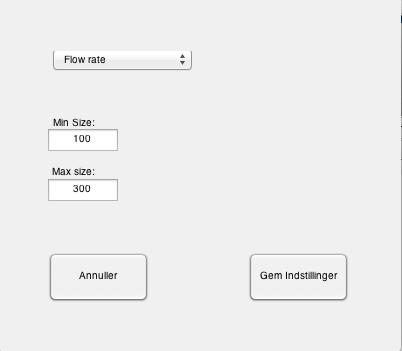
\includegraphics[width=0.5\textwidth]{billeder/GUI_settings.png}
	\caption{Mockup af Indstillinger}
	\label{fig:gui_settings}
\end{figure}


\newpage
\subsubsection{Callbacks}
For de 3 knapper i GUI'en oprettes der 3 callback funktioner, hvor forskellig kode eksekveres når knapperne klikkes. Disse 3 callback funktioner er nærmere beskrevet herunder bl.a. vha. flow chart diagrammer.
\subsubsection{Start Callback}
Denne callback funktion kaldes når operatøren klikker på Start knappen på GUI'en. Flowet i callbacket er vist i figur \ref{fig:act_start}.
\begin{figure}[H]
	\centering
	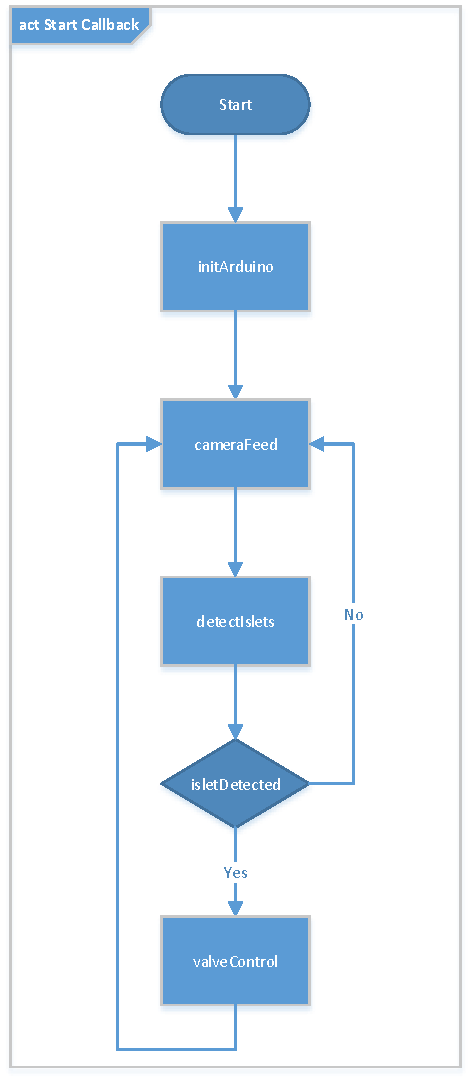
\includegraphics[width=0.5\textwidth]{billeder/act_start-crop.pdf}
	\caption{Flowchart diagram for Start Callback}
	\label{fig:act_start}
\end{figure}

\newpage
\subsubsection{Stop Callback}
Denne callback funktion kaldes når operatøren klikker på Stop knappen på GUI'en. Flowet i callbacket er vist i figur \ref{fig:act_stop}.
\begin{figure}[H]
	\centering
	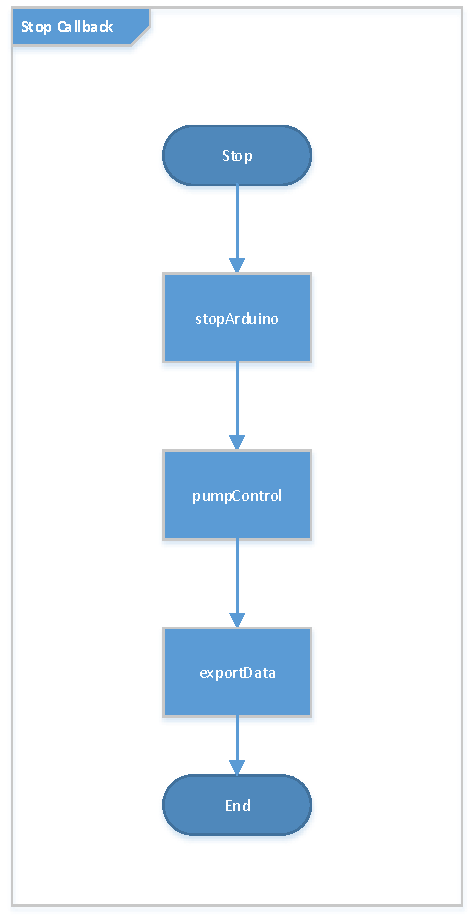
\includegraphics[width=0.5\textwidth]{billeder/act_stop-crop.pdf}
	\caption{Flowchart diagram for Stop Callback}
	\label{fig:act_stop}
\end{figure}

\newpage
\subsubsection{Indstillinger Callback}
Denne callback funktion kaldes når operatøren klikker på Settings knappen på GUI'en. Flowet i callbacket er vist i figur \ref{fig:act_settings}. Når knappen klikkes åbnes et nyt vindue, hvor systemets indstillinger kan ændres. De ændrede indstillinger anvendes i funktionerne detectIslets og pumpControl. 
\begin{figure}[H]
	\centering
	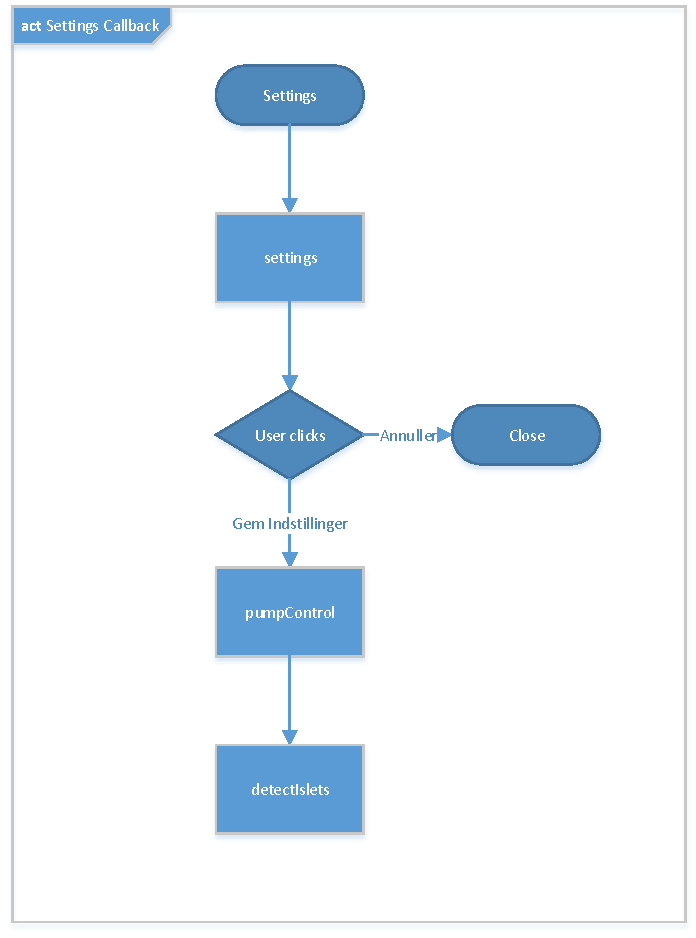
\includegraphics[width=0.5\textwidth]{billeder/act_settings-crop.pdf}
	\caption{Flowchart diagram for Settings Callback}
	\label{fig:act_settings}
\end{figure}








\section{Sekvensdiagrammer}
\subsection{Sekvensdiagram for usecase 1} 
\begin{figure}[H]
	\centering
	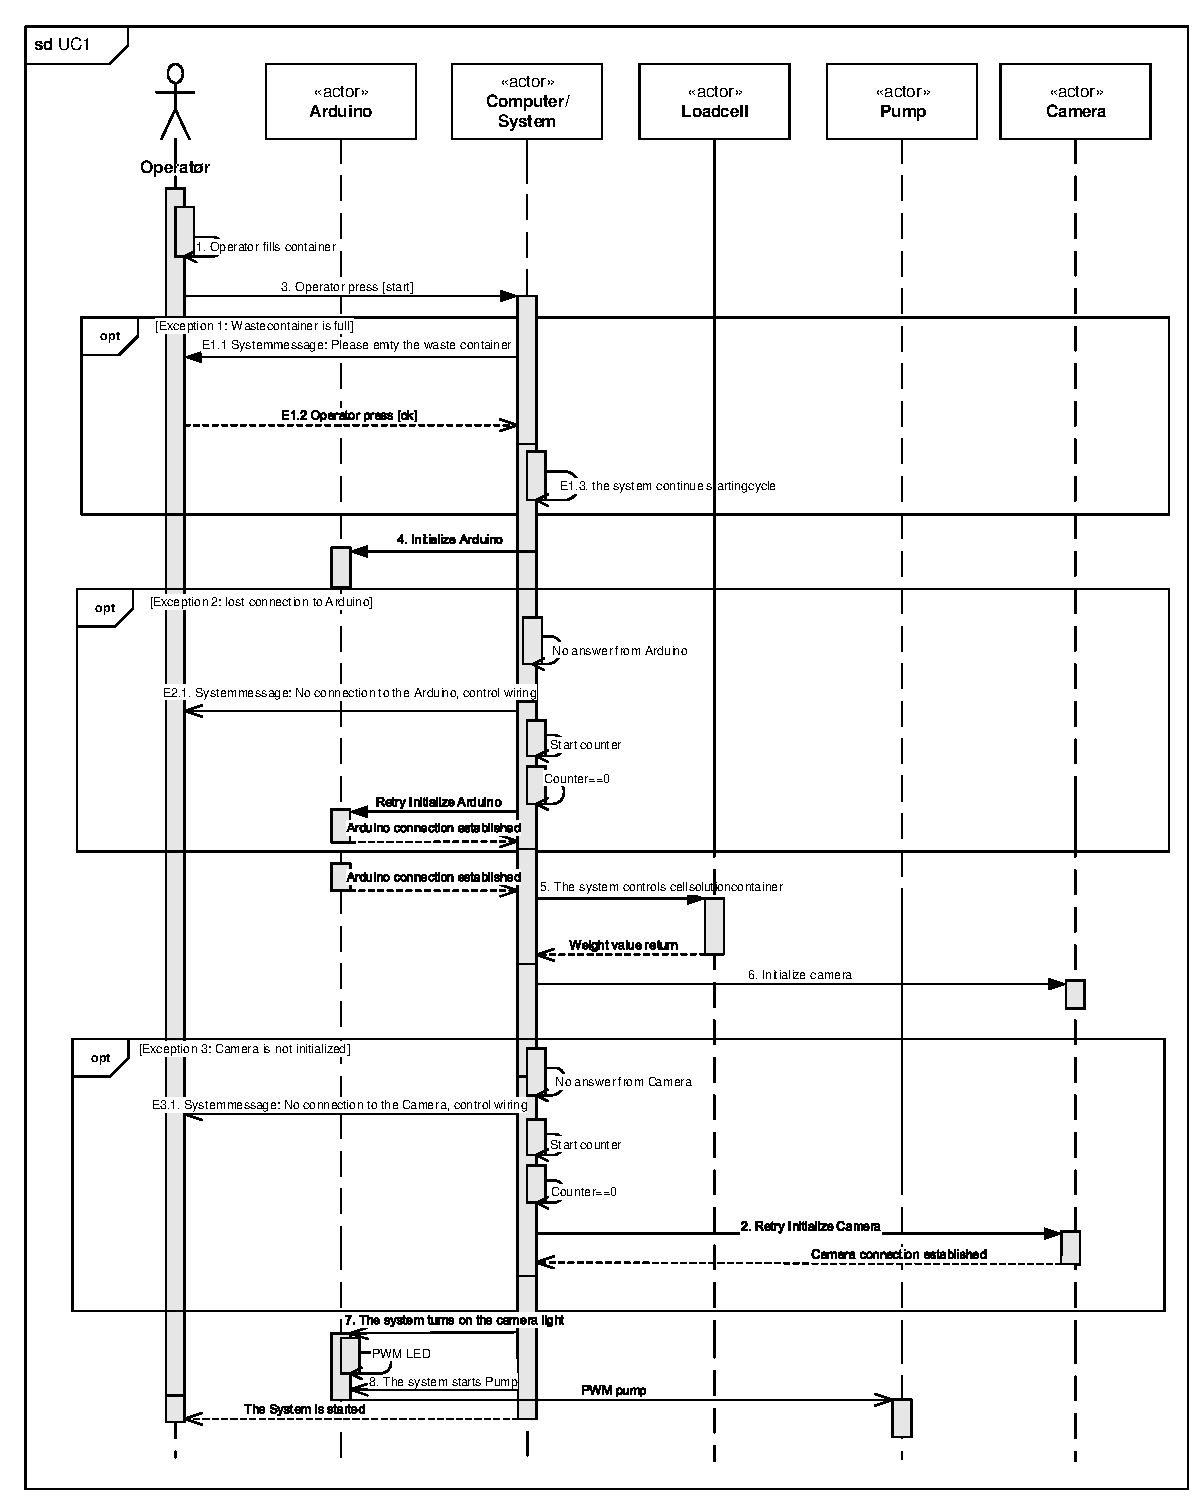
\includegraphics[width=1\textwidth]{pdf/UC1crop.pdf}
	\caption{Sekvensdiagram for usecase 1}
	\label{fig:uc1}
\end{figure}

\subsection{Sekvensdiagram for usecase 2} 
\begin{figure}[H]
	\centering
	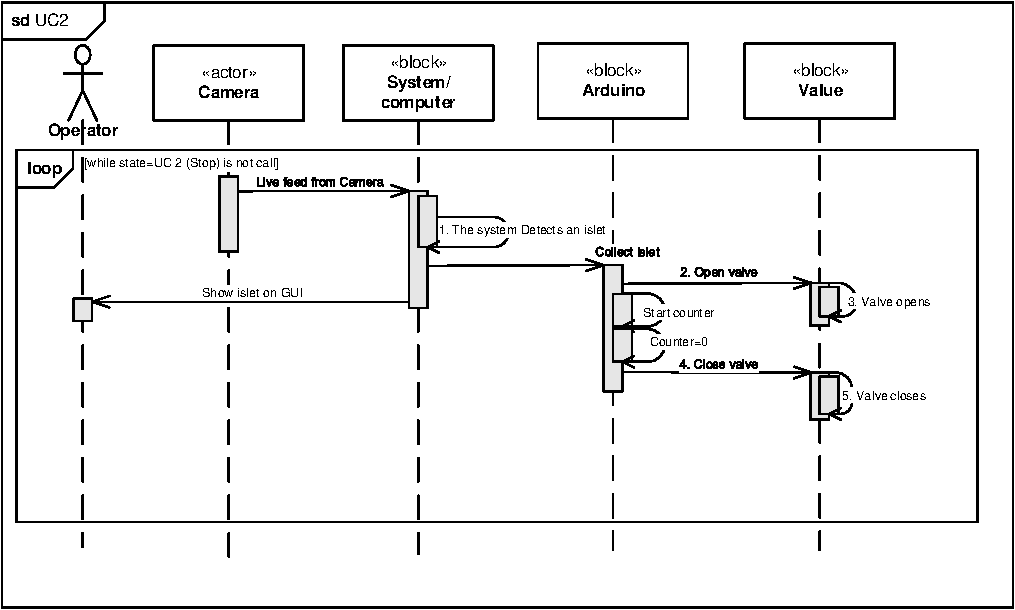
\includegraphics[width=1\textwidth]{pdf/UC2_cropped.pdf}
	\caption{Sekvensdiagram for usecase 2}
	\label{fig:uc1}
\end{figure}

\subsection{Sekvensdiagram for usecase 3} 
\begin{figure}[H]
	\centering
	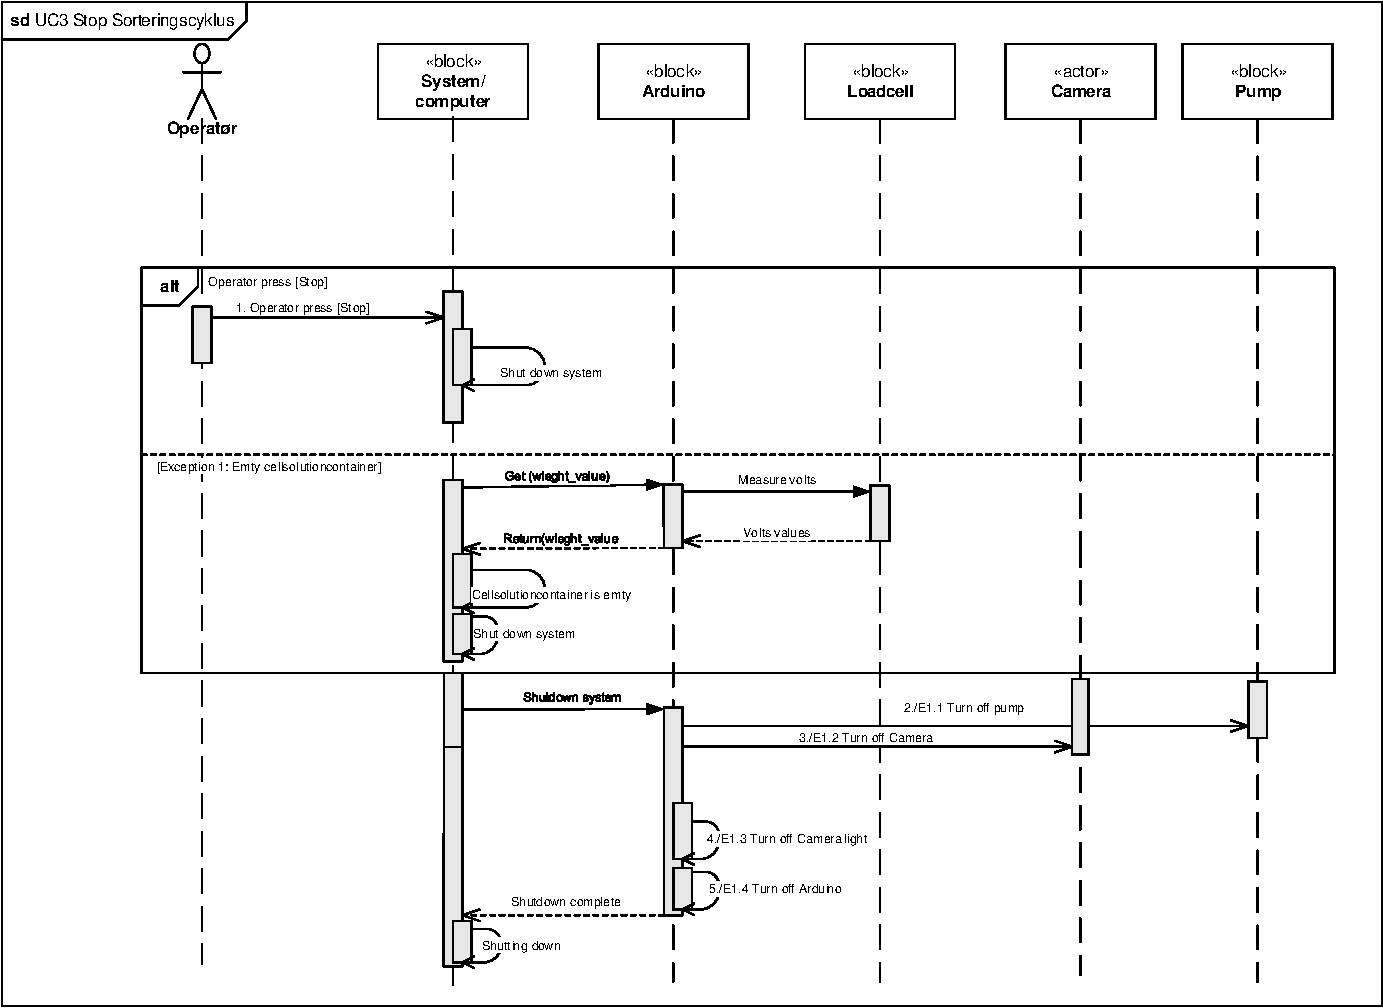
\includegraphics[width=1\textwidth]{pdf/UC3_cropped.pdf}
	\caption{Sekvensdiagram for usecase 3}
	\label{fig:uc1}
\end{figure}

\subsection{Sekvensdiagram for usecase 4} 
\begin{figure}[H]
	\centering
	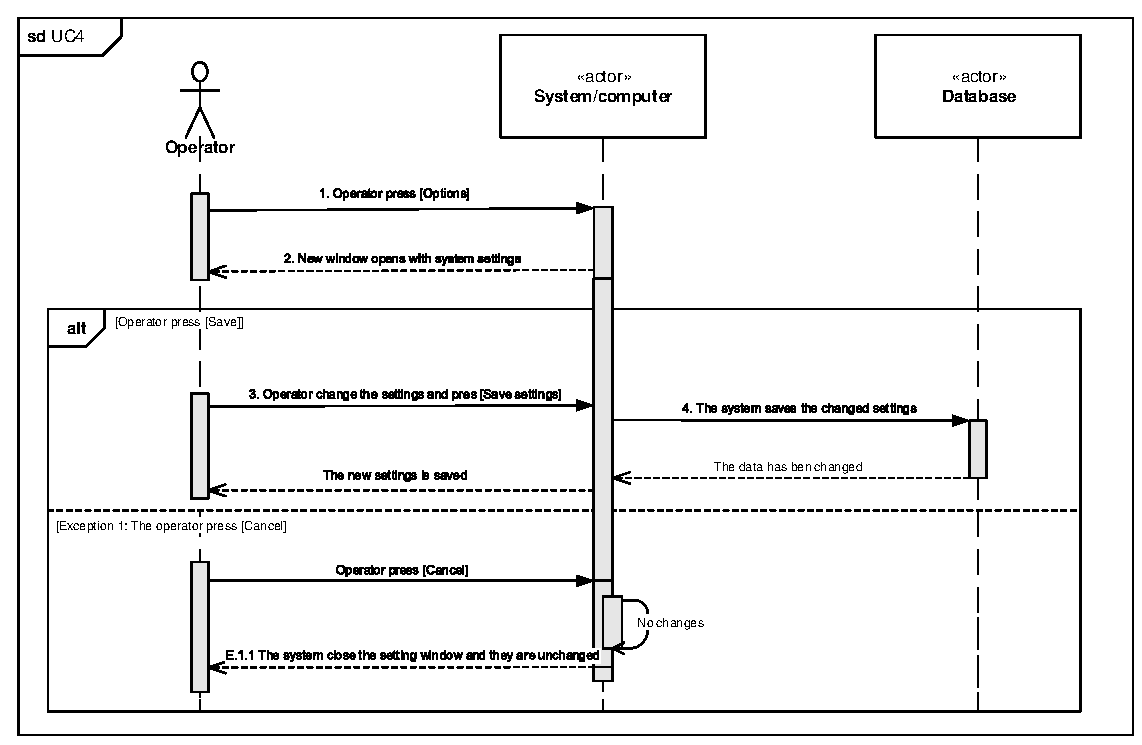
\includegraphics[width=1\textwidth]{pdf/UC4_cropped.pdf}
	\caption{Sekvensdiagram for usecase 4}
	\label{fig:uc1}
\end{figure}

\subsection{Sekvensdiagram for usecase 5} 
\begin{figure}[H]
	\centering
	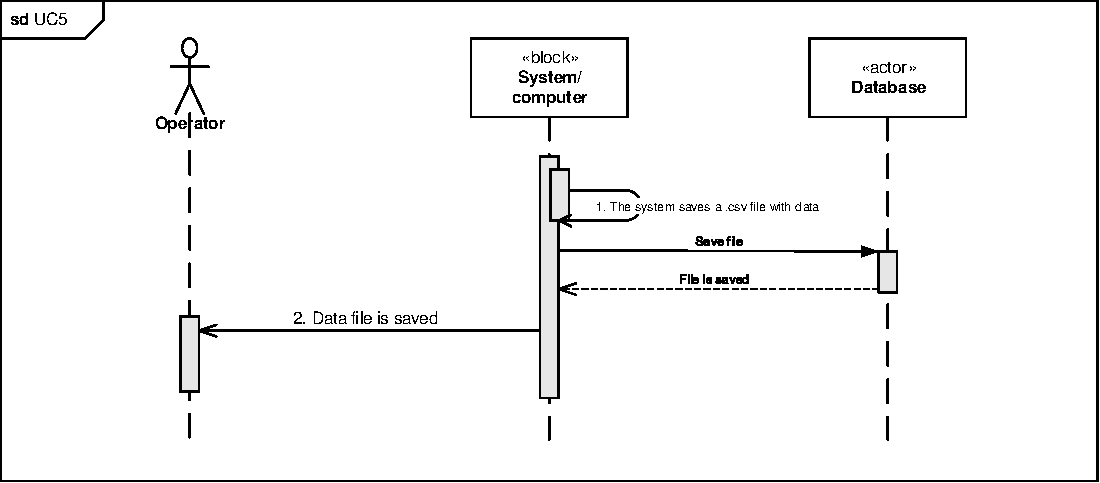
\includegraphics[width=1\textwidth]{pdf/UC5_cropped}
	\caption{Sekvensdiagram for usecase 5}
	\label{fig:uc1}
\end{figure}


%% Afrunding %%

%\section{Konklusion}
husk at problemformuleringenspunkter skal kunne afkrydses her nede


%%%% Kilder %%%%

\begingroup
	\raggedright
	\bibliography{bibtex/litteratur}							% Litteraturlisten inkluderes
\endgroup


%%%% Fixme-listen %%%%

\newpage														% Ny side til Fixme-listen
\listoffixmes													% Fixme-listen - fjernes til sidst i projektet med "%"


%%%% Appendiks %%%%

\appendix														% Appendiks/bilag start - giver chapter bogstaver i stedet for tal
\clearforchapter												% Sikrer at pagestylen aktiveres paa den rigtige side
\phantomsection													% Kunstigt afsnit, som hyperlinks kan 'holde fast i'
\pdfbookmark[0]{Appendiks}{appendiks}							% Tildeler en klikbar bookmark til den endelige PDF

%% Indstillinger for appendiks (deaktiveret med "%") %%

%\pagestyle{empty}												% Sidehoved/-fod for standardsider aendres til tom for appendiks
%\aliaspagestyle{chapter}{empty}								% Sidehoved/-fod for kapitelsider aendres til tom for appendiks
%\settocdepth{chapter}											% Kun kapitel-niveau vises i ToC
%\addtocontents{toc}{\protect\cftpagenumbersoff{chapter}}		% Sidetal for kapitler fjernes i ToC

%% Filer til appendiks %%

\chapter{Casehus} \label{sec:casehus}


%%%% Bilag %%%%

%\phantomsection												% Kunstigt afsnit, som hyperlinks kan 'holde fast i'
%\addcontentsline{toc}{chapter}{Bilag A \ Navn} 				% Manuelle indgange i indholdsfortegnelsen (naar \includepdf bruges)

%\includepdf[pages={x-y}]{filnavn}								% Inkluder eksterne bilag med \includepdf[pages={x-y}]{filnavn}


\end{document}													% Slutter dokumentet - obligatorisk


